% =====================================================================
%  Capítulo 11. Cointegración y modelos de corrección de errores
% =====================================================================
\chapter[Cointegración y VECM]{Cointegración y modelos vectoriales de corrección de errores}\label{cap:cointegracion}

\section*{Objetivos de aprendizaje}
Al terminar este capítulo, el lector podrá:
\begin{enumerate}[label=\arabic*.,leftmargin=*]
  \item Definir la cointegración y distinguirla de la regresión espuria.
  \item Reescribir un VAR en niveles como un modelo vectorial de corrección de errores (VECM) e interpretar sus
        matrices $\alpha$ y $\beta$.
  \item Aplicar la prueba de dos etapas de Engle y Granger y las pruebas de la traza y del máximo autovalor de
        Johansen, y contrastar restricciones sobre el vector de cointegración.
  \item Reconocer los cambios de régimen en una relación de largo plazo y evaluar si la corrección de errores
        mejora los pronósticos.
\end{enumerate}

\section*{Motivación}
El Capítulo~\ref{cap:raiz} mostró que los precios suelen tener raíz unitaria y que regresar un paseo aleatorio
sobre otro independiente produce relaciones espurias. Pero hay precios que \emph{no} son independientes: el
petróleo Brent y el WTI son casi el mismo producto, y si uno se encarece mucho respecto del otro, los
comerciantes compran el barato y venden el caro hasta cerrar la brecha. Cada precio deambula sin rumbo fijo,
pero la diferencia entre ellos se mantiene acotada. Esa idea, la \emph{cointegración} (Engle y Granger, 1987),
describe muchas relaciones financieras: el precio al contado y el de futuros, las tasas de interés de distintos
plazos, los precios de un mismo activo en dos mercados y, según la teoría, el precio de una acción y sus
dividendos.

\paragraph{Datos del capítulo.} Promedios mensuales de los precios diarios del Brent y del WTI de la EIA de
EE.\,UU.\ (mayo de 1987 a octubre de 2026, $T=474$) y datos anuales de precios, dividendos y utilidades reales del
S\&P 500 de la base de Shiller (1871--2023). Usamos promedios mensuales porque el 20 de abril de 2020 el WTI
cerró en $-36{,}98$ dólares, un precio negativo cuyo logaritmo no existe; los promedios mensuales son siempre
positivos.

% ---------------------------------------------------------------------
\section{Cointegración}
% ---------------------------------------------------------------------

\begin{definicion}[Cointegración; Engle y Granger, 1987]
Las componentes del vector $\mathbf y_t$ ($K\times1$) están \emph{cointegradas} si cada una es I(1) y existe un
vector $\boldsymbol\beta\ne\mathbf 0$ tal que $\boldsymbol\beta'\mathbf y_t$ es I(0). El vector
$\boldsymbol\beta$ es un \emph{vector de cointegración}, y $\boldsymbol\beta'\mathbf y_t$ la \emph{relación de
equilibrio}. El número de vectores de cointegración linealmente independientes, $r$, es el \emph{rango de
cointegración}; $0<r<K$.
\end{definicion}

Un modelo sencillo con $K=2$ lo ilustra. Sea $w_t$ un paseo aleatorio, la tendencia común, y $z_t$ un proceso
estacionario. Si
\begin{align*}
  y_{1t} &= w_t+\tfrac12 z_t,\\
  y_{2t} &= w_t-\tfrac12 z_t,
\end{align*}
cada precio hereda la raíz unitaria de $w_t$, pero
\begin{align*}
  y_{1t}-y_{2t} &= \bigl(w_t+\tfrac12z_t\bigr)-\bigl(w_t-\tfrac12z_t\bigr)\\
                &= z_t,
\end{align*}
que es estacionario: $\boldsymbol\beta=(1,-1)'$. La Figura~\ref{fig:cointsim} contrasta este caso con dos
paseos aleatorios independientes, cuya diferencia es otro paseo aleatorio que se aleja sin volver.

\begin{figure}[ht]
\centering
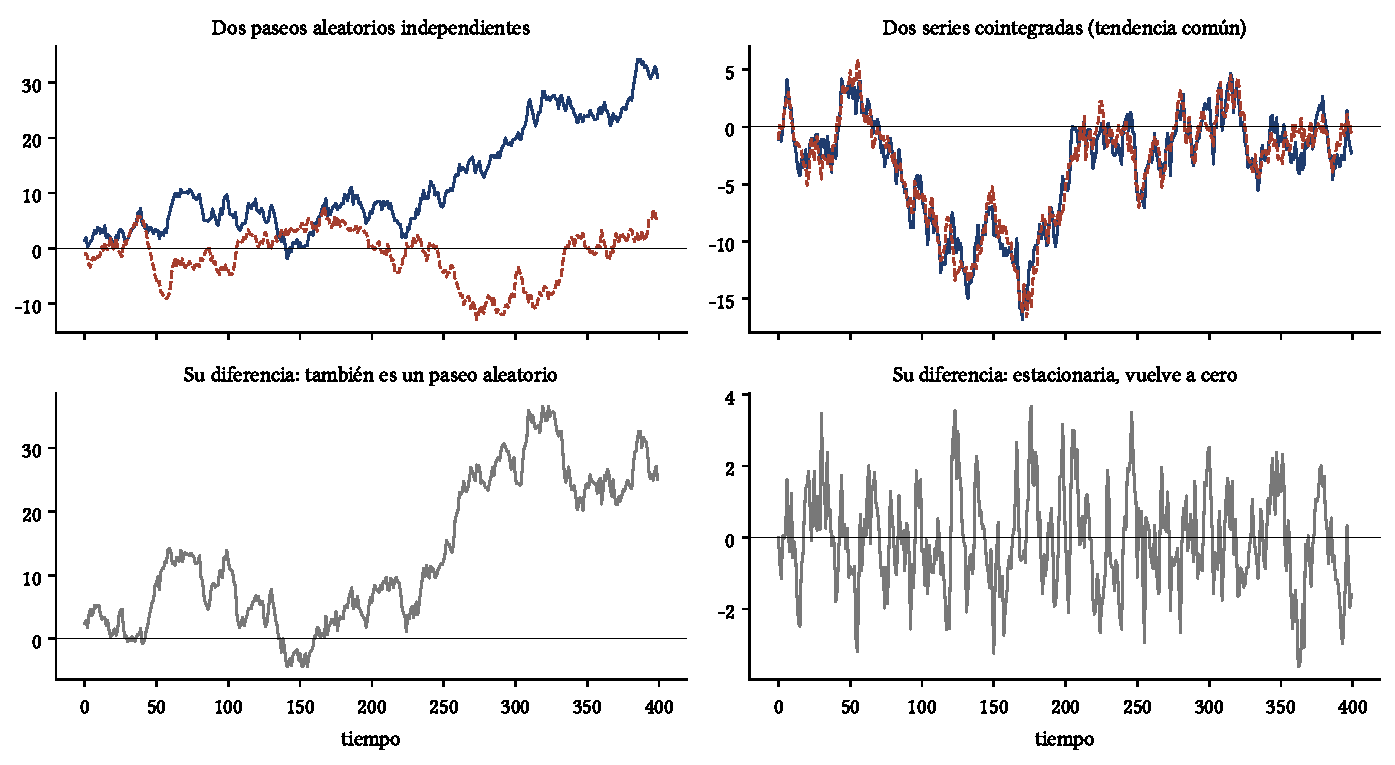
\includegraphics[width=\linewidth]{graficos/cap11_fig_coint_sim.pdf}
\caption{Izquierda: dos paseos aleatorios independientes y su diferencia, que no tiene nivel al que regresar.
Derecha: dos series cointegradas con una tendencia común y su diferencia, que fluctúa alrededor de cero.}
\label{fig:cointsim}
\end{figure}

% ---------------------------------------------------------------------
\section{El modelo vectorial de corrección de errores}
% ---------------------------------------------------------------------

\begin{proposicion}[Del VAR al VECM]\label{prop:vecm}
Todo VAR($p$) en niveles,
$\mathbf y_t=\mathbf c+A_1\mathbf y_{t-1}+\dots+A_p\mathbf y_{t-p}+\mathbf u_t$, puede escribirse como
\[
  \Delta\mathbf y_t=\mathbf c+\Pi\,\mathbf y_{t-1}+\sum_{i=1}^{p-1}\Gamma_i\,\Delta\mathbf y_{t-i}+\mathbf u_t,
\]
con $\Pi=-(I_K-A_1-\dots-A_p)$ y $\Gamma_i=-(A_{i+1}+\dots+A_p)$.
\end{proposicion}

\begin{proof}
Lo mostramos para $p=2$; el caso general sigue el mismo procedimiento. Restamos $\mathbf y_{t-1}$ a ambos lados,
y sumamos y restamos $A_2\mathbf y_{t-1}$ en el lado derecho:
\begin{align*}
  \mathbf y_t-\mathbf y_{t-1} &= \mathbf c+A_1\mathbf y_{t-1}-\mathbf y_{t-1}+A_2\mathbf y_{t-2}+\mathbf u_t\\
                              &= \mathbf c+(A_1-I_K)\mathbf y_{t-1}+A_2\mathbf y_{t-1}-A_2\mathbf y_{t-1}+A_2\mathbf y_{t-2}+\mathbf u_t\\
                              &= \mathbf c+(A_1+A_2-I_K)\mathbf y_{t-1}-A_2(\mathbf y_{t-1}-\mathbf y_{t-2})+\mathbf u_t,\\[4pt]
  \Delta\mathbf y_t           &= \mathbf c+\Pi\,\mathbf y_{t-1}+\Gamma_1\Delta\mathbf y_{t-1}+\mathbf u_t,
\end{align*}
con $\Pi=-(I_K-A_1-A_2)$ y $\Gamma_1=-A_2$.
\end{proof}

El rango de $\Pi$ determina el tipo de sistema:
\begin{itemize}[leftmargin=*]
  \item $\operatorname{rango}(\Pi)=K$: $\Pi$ es invertible, y $\mathbf y_{t-1}=\Pi^{-1}(\Delta\mathbf y_t-\dots)$ es
        estacionario porque el lado derecho lo es. Todas las variables son I(0).
  \item $\operatorname{rango}(\Pi)=0$: $\Pi=0$ y el modelo es un VAR en primeras diferencias. No hay cointegración.
  \item $0<\operatorname{rango}(\Pi)=r<K$: $\Pi$ se factoriza como $\Pi=\alpha\beta'$, con $\alpha$ y $\beta$ de
        dimensión $K\times r$. Como $\Delta\mathbf y_t$ es estacionario, también debe serlo
        $\alpha\beta'\mathbf y_{t-1}$, y por tanto $\beta'\mathbf y_{t-1}$: hay $r$ relaciones de
        cointegración.
\end{itemize}

En el tercer caso el modelo es el \emph{VECM}:
\[
  \Delta\mathbf y_t=\mathbf c+\alpha\,\bigl(\beta'\mathbf y_{t-1}\bigr)+\sum_{i=1}^{p-1}\Gamma_i\Delta\mathbf y_{t-i}+\mathbf u_t .
\]
El término $\beta'\mathbf y_{t-1}$ mide el desequilibrio del período anterior, y $\alpha$ contiene las
\emph{velocidades de ajuste}: cuánto corrige cada variable ante ese desequilibrio. Si $\beta=(1,-1)'$ y el
desequilibrio es positivo ($y_1$ caro respecto de $y_2$), la corrección exige $\alpha_1<0$ (que $y_1$ baje),
$\alpha_2>0$ (que $y_2$ suba) o ambas. Una variable con $\alpha_i=0$ es \emph{débilmente exógena}: no reacciona al
desequilibrio y es la que ``lidera'' el precio común.

\begin{proposicion}[Persistencia del desequilibrio y tendencia común]\label{prop:ajustevecm}
Sea un VECM bivariado sin rezagos ni constante,
$\Delta\mathbf y_t=\alpha\beta'\mathbf y_{t-1}+\mathbf u_t$, con $\beta=(1,-1)'$ y $\alpha=(\alpha_1,\alpha_2)'$.
Entonces:
\begin{enumerate}[label=(\roman*)]
  \item el desequilibrio $z_t=\beta'\mathbf y_t$ sigue un AR(1) con coeficiente $1+\beta'\alpha=1+\alpha_1-\alpha_2$;
  \item sin nuevos choques, ambas variables convergen a un nivel común; tras un choque inicial
        $\mathbf y_0=(1,0)'$, ese nivel es $\alpha_2/(\alpha_2-\alpha_1)$.
\end{enumerate}
\end{proposicion}

\begin{proof}
(i) Multiplicamos el modelo por $\beta'$:
\begin{align*}
  \beta'\mathbf y_t-\beta'\mathbf y_{t-1} &= \beta'\alpha\,\beta'\mathbf y_{t-1}+\beta'\mathbf u_t,\\
  z_t &= (1+\beta'\alpha)\,z_{t-1}+\beta'\mathbf u_t,\\
  1+\beta'\alpha &= 1+\alpha_1-\alpha_2 .
\end{align*}
(ii) El vector $\alpha_\perp=(\alpha_2,-\alpha_1)'$ cumple $\alpha_\perp'\alpha=\alpha_2\alpha_1-\alpha_1\alpha_2=0$.
Multiplicando el modelo sin choques por $\alpha_\perp'$:
\begin{align*}
  \alpha_\perp'\Delta\mathbf y_t &= \alpha_\perp'\alpha\,\beta'\mathbf y_{t-1}\\
                                 &= 0 .
\end{align*}
La combinación $\alpha_\perp'\mathbf y_t=\alpha_2y_{1t}-\alpha_1y_{2t}$ no cambia nunca: es la tendencia común.
Al inicio vale $\alpha_2\cdot1-\alpha_1\cdot0=\alpha_2$. Al final el desequilibrio desaparece y
$y_1=y_2=\ell$, así que
\begin{align*}
  \alpha_2\ell-\alpha_1\ell &= \alpha_2,\\
  \ell &= \frac{\alpha_2}{\alpha_2-\alpha_1}. && \qedhere
\end{align*}
\end{proof}

La Figura~\ref{fig:ajuste} muestra la proposición con $1+\beta'\alpha=0{,}75$ en los dos casos. Con
$\alpha=(-0{,}05;\,0{,}20)$ casi todo el ajuste lo hace $y_2$, y el nivel final es $0{,}20/0{,}25=0{,}8$: el choque a
$y_1$ es en su mayor parte permanente. Con $\alpha=(-0{,}20;\,0{,}05)$, el ajuste lo hace $y_1$ y el nivel final es
$0{,}05/0{,}25=0{,}2$: el choque se deshace casi por completo. La variable que no ajusta es la que fija el precio.

\begin{figure}[ht]
\centering
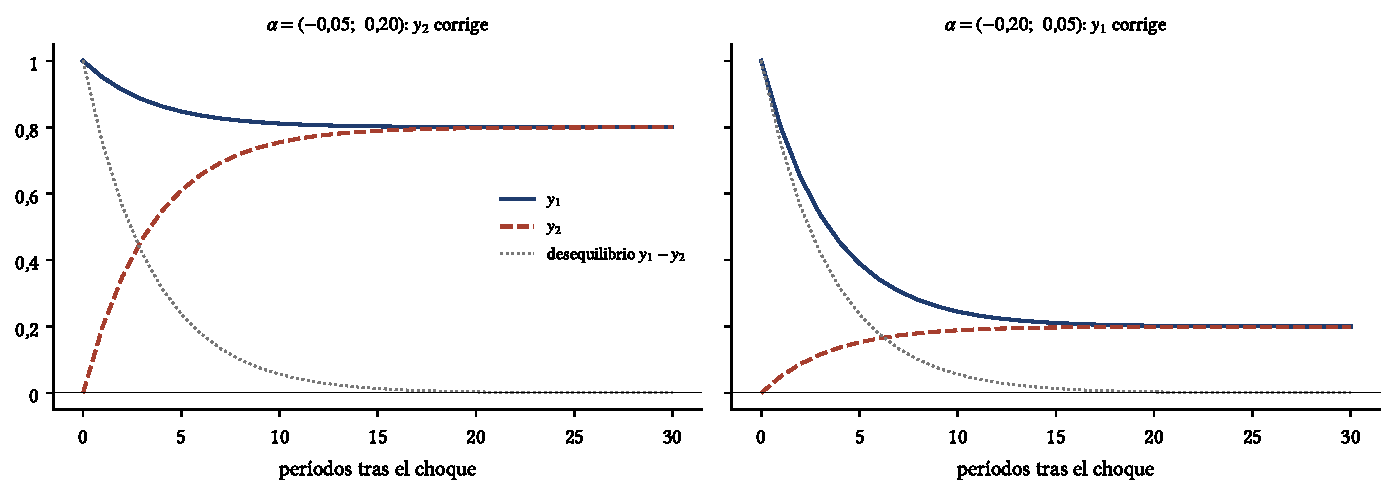
\includegraphics[width=\linewidth]{graficos/cap11_fig_ajuste.pdf}
\caption{Respuesta de un VECM bivariado con $\beta=(1,-1)'$ a un choque de $+1$ en $y_1$. Ambas variables
convergen a un nivel común; quién ajusta lo deciden los coeficientes $\alpha$.}
\label{fig:ajuste}
\end{figure}

% ---------------------------------------------------------------------
\section{El método de dos etapas de Engle y Granger}
% ---------------------------------------------------------------------

Con $K=2$ y a lo sumo una relación de cointegración, Engle y Granger (1987) proponen:
\begin{enumerate}[leftmargin=*]
  \item Estimar por MCO la regresión de cointegración $y_{1t}=a+b\,y_{2t}+u_t$.
  \item Aplicar una prueba ADF \emph{sin constante} a los residuos $\hat u_t$:
        $\Delta\hat u_t=\gamma\hat u_{t-1}+\sum_j\delta_j\Delta\hat u_{t-j}+e_t$. Si $\gamma<0$ es significativo,
        los residuos son estacionarios y las series están cointegradas.
\end{enumerate}

Hay dos sutilezas. Primero, el estimador de $b$ es \emph{superconsistente}: converge a una velocidad $T$ en
lugar de $\sqrt T$. La razón es que el regresor I(1) tiene una varianza muestral que crece con $T$: si $b$ fuera
incorrecto, los residuos serían I(1) y su suma de cuadrados crecería como $T^2$, mientras que con el $b$
correcto crece solo como $T$. Minimizar la suma de cuadrados ``encuentra'' el $b$ correcto muy rápido, aunque
$u_t$ esté correlacionado con $y_{2t}$. Segundo, los valores críticos de la prueba ADF \emph{no} son los de
Dickey y Fuller: como $\hat b$ se eligió para que los residuos parezcan lo más estacionarios posible, la prueba
rechaza con más facilidad, y hay que exigir más. MacKinnon (2010) da superficies de respuesta
$c(T)=b_\infty+b_1/T+b_2/T^2$; con dos variables y constante, el valor crítico asintótico al 5\,\% es $-3{,}34$, en
lugar de $-2{,}86$.

El método tiene limitaciones: el resultado puede depender de qué variable se pone a la izquierda, no permite
probar más de una relación y no ofrece una prueba directa sobre $b$, porque la distribución de $\hat b$ no es
estándar. El método de Johansen resuelve los tres problemas.

% ---------------------------------------------------------------------
\section{El método de Johansen}
% ---------------------------------------------------------------------

Johansen (1988, 1991) estima el VECM por máxima verosimilitud con la restricción de rango
$\Pi=\alpha\beta'$. Sean $R_{0t}$ y $R_{1t}$ los residuos de regresar, respectivamente, $\Delta\mathbf y_t$ y
$\mathbf y_{t-1}$ sobre la constante y los rezagos $\Delta\mathbf y_{t-1},\dots,\Delta\mathbf y_{t-p+1}$, y
\[
  S_{ij}=\frac1n\sum_{t}R_{it}R_{jt}',\qquad i,j\in\{0,1\}.
\]

\begin{proposicion}[Estimador y prueba de la traza de Johansen]\label{prop:johansen}
Sean $\hat\lambda_1>\dots>\hat\lambda_K$ los autovalores de $S_{11}^{-1}S_{10}S_{00}^{-1}S_{01}$ y
$\hat{\mathbf v}_i$ sus autovectores, normalizados con $\hat{\mathbf v}_i'S_{11}\hat{\mathbf v}_i=1$. Con rango $r$:
\begin{enumerate}[label=(\roman*)]
  \item $\hat\beta=(\hat{\mathbf v}_1,\dots,\hat{\mathbf v}_r)$ y $\hat\alpha=S_{01}\hat\beta$;
  \item la verosimilitud máxima cumple $L_{\max}^{-2/n}\propto|S_{00}|\prod_{i=1}^{r}(1-\hat\lambda_i)$;
  \item el estadístico de razón de verosimilitudes de $H_0$: rango $\le r$ frente a rango $=K$ es
        \[
          \lambda_{\text{traza}}(r)=-n\sum_{i=r+1}^{K}\ln\bigl(1-\hat\lambda_i\bigr).
        \]
\end{enumerate}
\end{proposicion}

\begin{proof}
Por el teorema de Frisch-Waugh-Lovell, una vez concentrados los parámetros de corto plazo, el modelo es
$R_{0t}=\alpha\beta'R_{1t}+\mathbf u_t$. Para $\beta$ fijo, es una regresión de $R_{0t}$ sobre
$\beta'R_{1t}$, con soluciones
\begin{align*}
  \hat\alpha(\beta)  &= S_{01}\beta\,(\beta'S_{11}\beta)^{-1},\\
  \hat\Sigma(\beta) &= S_{00}-S_{01}\beta\,(\beta'S_{11}\beta)^{-1}\beta'S_{10}.
\end{align*}
Con errores normales, la verosimilitud concentrada cumple $L_{\max}^{-2/n}\propto|\hat\Sigma(\beta)|$. Usamos la
identidad de determinantes de matrices por bloques,
$|A|\,|D-CA^{-1}B|=|D|\,|A-BD^{-1}C|$, con $A=S_{00}$, $B=S_{01}\beta$, $C=\beta'S_{10}$ y $D=\beta'S_{11}\beta$:
\begin{align*}
  |\hat\Sigma(\beta)| &= \bigl|S_{00}-S_{01}\beta(\beta'S_{11}\beta)^{-1}\beta'S_{10}\bigr|\\
                      &= |S_{00}|\,\frac{\bigl|\beta'S_{11}\beta-\beta'S_{10}S_{00}^{-1}S_{01}\beta\bigr|}{|\beta'S_{11}\beta|}\\
                      &= |S_{00}|\,\frac{\bigl|\beta'\bigl(S_{11}-S_{10}S_{00}^{-1}S_{01}\bigr)\beta\bigr|}{|\beta'S_{11}\beta|}.
\end{align*}
Minimizar un cociente de determinantes de este tipo es un problema de autovalores generalizados: el mínimo se
alcanza con las columnas de $\beta$ iguales a los autovectores de
$\bigl|\lambda S_{11}-S_{10}S_{00}^{-1}S_{01}\bigr|=0$ con los $r$ autovalores mayores. Con la normalización
$\beta'S_{11}\beta=I_r$, se tiene $\beta'S_{10}S_{00}^{-1}S_{01}\beta=\operatorname{diag}(\hat\lambda_1,\dots,\hat\lambda_r)$ y
\begin{align*}
  |\hat\Sigma(\hat\beta)| &= |S_{00}|\,\frac{\bigl|I_r-\operatorname{diag}(\hat\lambda_1,\dots,\hat\lambda_r)\bigr|}{|I_r|}\\
                          &= |S_{00}|\prod_{i=1}^{r}(1-\hat\lambda_i),
\end{align*}
y $\hat\alpha=S_{01}\hat\beta(\hat\beta'S_{11}\hat\beta)^{-1}=S_{01}\hat\beta$. La razón de verosimilitudes entre
el rango $r$ y el rango completo $K$ es entonces
\begin{align*}
  -2\ln\frac{L_{\max}(r)}{L_{\max}(K)} &= n\ln\frac{|S_{00}|\prod_{i=1}^{r}(1-\hat\lambda_i)}{|S_{00}|\prod_{i=1}^{K}(1-\hat\lambda_i)}\\
                                       &= -n\sum_{i=r+1}^{K}\ln(1-\hat\lambda_i). && \qedhere
\end{align*}
\end{proof}

Los autovalores son las correlaciones canónicas al cuadrado entre $\Delta\mathbf y_t$ y $\mathbf y_{t-1}$, una
vez descontada la dinámica de corto plazo: un $\hat\lambda_i$ cercano a cero indica una combinación de niveles que
no ayuda a explicar los cambios, es decir, que no es una relación de equilibrio. La prueba se aplica en
secuencia: se contrasta $r=0$; si se rechaza, $r\le1$, y así hasta no rechazar. El estadístico del \emph{máximo
autovalor}, $\lambda_{\max}(r)=-n\ln(1-\hat\lambda_{r+1})$, contrasta rango $r$ frente a $r+1$. Las distribuciones
no son estándar y dependen de los términos deterministas; usamos los valores críticos de MacKinnon, Haug y
Michelis (1999) para el caso de constante sin restringir. Con $K-r=1$, el valor al 5\,\% es $3{,}84$; con $K-r=2$,
$15{,}49$ para la traza y $14{,}26$ para el máximo autovalor.

\paragraph{Restricciones sobre $\beta$.} La hipótesis $\beta=H\boldsymbol\varphi$, con $H$ una matriz conocida
$K\times s$ (por ejemplo, $H=(1,-1)'$ para una relación uno a uno), se contrasta resolviendo el mismo problema de
autovalores con $H'S_{11}H$ y $S_{01}H$ en lugar de $S_{11}$ y $S_{01}$. Si $\tilde\lambda_1$ es el mayor autovalor
restringido, con $r=1$
\[
  LR=n\,\bigl[\ln(1-\tilde\lambda_1)-\ln(1-\hat\lambda_1)\bigr]\ \xrightarrow{d}\ \chi^2_{K-s}.
\]
A diferencia de las pruebas de rango, esta sí tiene distribución estándar.

% ---------------------------------------------------------------------
\section{Ejercicios resueltos}
% ---------------------------------------------------------------------

\begin{ejresuelto}{¿Están cointegrados el Brent y el WTI?}\label{ej:eg}
\enunciado Con los logaritmos de los precios promedio mensuales del Brent ($B_t$) y del WTI ($W_t$), verifique que
ambos son I(1) y aplique la prueba de Engle y Granger en las dos direcciones.

\solucion
\paso{Paso 1. Orden de integración.} Con la función \texttt{adf} del Capítulo~\ref{cap:raiz} (rezagos por AIC):
\begin{center}\small
\begin{tabular}{@{}lrr@{}}
\toprule
Serie & Nivel: $t$ (rezagos) & Diferencia: $t$ (rezagos) \\
\midrule
$\log$ Brent & $-1{,}37$ (4) & $-12{,}28$ (3) \\
$\log$ WTI   & $-1{,}54$ (4) & $-12{,}25$ (3) \\
\bottomrule
\end{tabular}
\end{center}
Con un valor crítico de $-2{,}86$, no se rechaza la raíz unitaria en niveles y se rechaza con holgura en
diferencias: ambas series son I(1).

\paso{Paso 2. Regresión de cointegración.} Por MCO,
\begin{align*}
  \hat B_t &= -0{,}3529+1{,}0943\,W_t .
\end{align*}
Los errores estándar de MCO no son válidos aquí, así que no los reportamos.

\paso{Paso 3. ADF sobre los residuos.} Con 2 rezagos (AIC), $\hat\gamma=-0{,}1467$ y $t=-5{,}338$. El valor crítico
al 5\,\% de MacKinnon para $T=474$ es
\begin{align*}
  c(474) &= -3{,}33613-\frac{6{,}1101}{474}-\frac{6{,}823}{474^2}\\
         &= -3{,}33613-0{,}01289-0{,}00003\\
         &= -3{,}349 .
\end{align*}
Como $-5{,}338<-3{,}349$ (y también $<-3{,}920$, el valor al 1\,\%), se rechaza la hipótesis de no cointegración.
En la otra dirección ($W_t$ sobre $B_t$), $t=-5{,}409$: la conclusión no depende de la normalización.

\paso{Paso 4. Velocidad de corrección.} El coeficiente autorregresivo del residuo es
$1+\hat\gamma=0{,}8533$, de modo que la vida media del desequilibrio es aproximadamente
\begin{align*}
  h_{1/2} &= \frac{\ln0{,}5}{\ln0{,}8533}\\
          &= 4{,}4\ \text{meses}.
\end{align*}
El residuo tiene desviación estándar de $0{,}055$ (unos 5,5\,\% de diferencia de precio); su mínimo, $-0{,}154$, ocurre
en septiembre de 2008 y su máximo, $0{,}213$, en abril de 2020, cuando el WTI se desplomó por la falta de
almacenamiento en EE.\,UU.\ (Figura~\ref{fig:brentwti}).

\codigoweb{cap11_ej01}
\salidaR{cap11_ej01_R.txt}
\lectura{cap11_ej01}

\RvsPy La prueba ADF de los residuos usa la opción \texttt{det = "n"} (sin términos deterministas) de la función
del Capítulo~\ref{cap:raiz}, porque los residuos de MCO ya tienen media cero. En Python, \texttt{coint} de
\texttt{statsmodels} reproduce el estadístico ($-5{,}338$) y los valores críticos, que calcula con la misma
superficie de respuesta de MacKinnon (2010). Los promedios mensuales se calculan con \texttt{aggregate} en R y
con \texttt{groupby} en \texttt{pandas}.

\begin{figure}[ht]
\centering
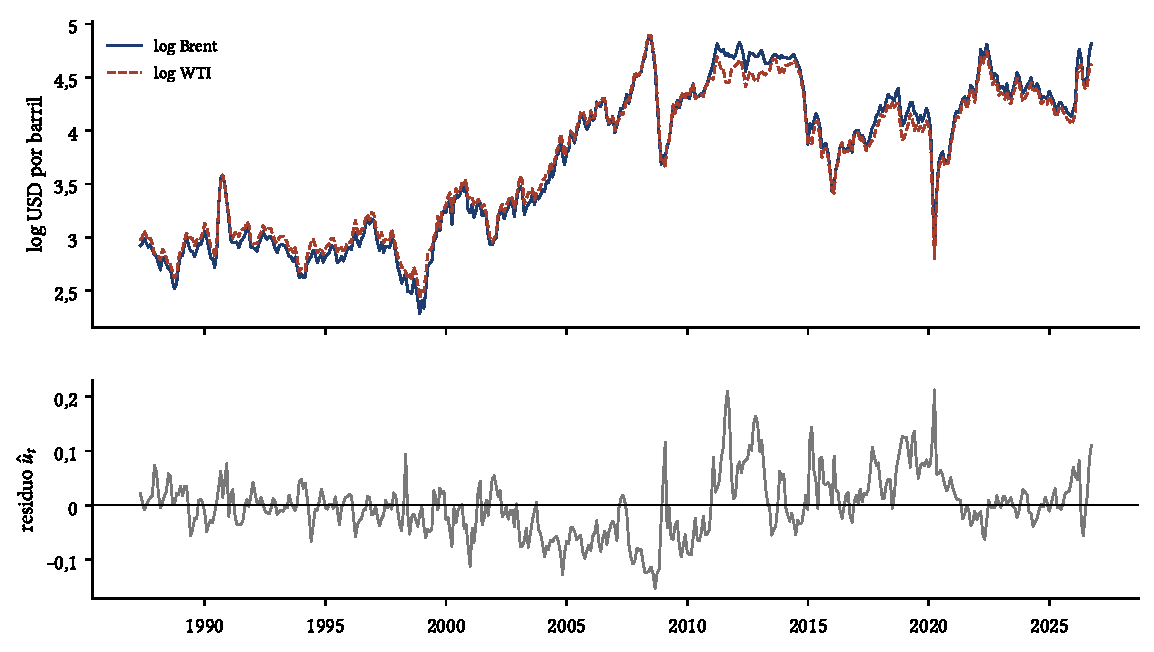
\includegraphics[width=0.92\linewidth]{graficos/cap11_ej01_brent_wti.pdf}
\caption{Arriba: logaritmos de los precios promedio mensuales del Brent y del WTI. Abajo: residuo de la regresión
de cointegración, que fluctúa alrededor de cero.}
\label{fig:brentwti}
\end{figure}

\begin{conclusion}
El Brent y el WTI están cointegrados: cada precio es un paseo aleatorio, pero la brecha entre ellos se corrige con
una vida media de unos cuatro meses.
\end{conclusion}
\end{ejresuelto}

\begin{ejresuelto}{Prueba de Johansen y VECM del petróleo}\label{ej:johansen}
\enunciado Elija el número de rezagos de un VAR en niveles con el BIC, aplique las pruebas de Johansen, estime el
VECM con $r=1$ e interprete $\hat\alpha$. Contraste $\beta=(1,-1)'$.

\solucion
\paso{Paso 1. Rezagos.} El BIC (y también el AIC) elige un VAR(3) en niveles, es decir, $k=2$ rezagos de las
diferencias en el VECM.

\paso{Paso 2. Rango.} Los autovalores son $\hat\lambda_1=0{,}06311$ y $\hat\lambda_2=0{,}00497$, con $n=471$:
\begin{align*}
  \lambda_{\text{traza}}(0) &= -471\bigl[\ln(1-0{,}06311)+\ln(1-0{,}00497)\bigr]\\
                            &= -471\,(-0{,}06519-0{,}00499)\\
                            &= 33{,}05,\\[4pt]
  \lambda_{\text{traza}}(1) &= -471\ln(1-0{,}00497)=2{,}35 .
\end{align*}
\begin{center}\small
\begin{tabular}{@{}lrrrr@{}}
\toprule
$H_0$ & Traza & VC 95\,\% & Máximo autovalor & VC 95\,\% \\
\midrule
$r=0$     & 33,05 & 15,49 & 30,70 & 14,26 \\
$r\le1$   & 2,35  & 3,84  & 2,35  & 3,84 \\
\bottomrule
\end{tabular}
\end{center}
Se rechaza $r=0$ y no se rechaza $r\le1$: hay exactamente una relación de cointegración.

\paso{Paso 3. VECM.} Normalizando el primer elemento a uno, $\hat\beta=(1;\ -1{,}1119)$, y
\begin{align*}
  \hat\alpha_{\text{Brent}} &= 0{,}0342\quad(t=0{,}40),\\
  \hat\alpha_{\text{WTI}}   &= 0{,}1664\quad(t=2{,}03).
\end{align*}
Solo el WTI corrige el desequilibrio: cuando el Brent está caro respecto del WTI, es el WTI el que sube al mes
siguiente. El Brent es débilmente exógeno, es decir, el precio de referencia que lidera. Es coherente con el
papel del Brent como marcador internacional, que fija el precio de dos tercios del crudo comerciado en el mundo.

\paso{Paso 4. Persistencia.} Por la Proposición~\ref{prop:ajustevecm}, aplicada como aproximación a un modelo con
rezagos:
\begin{align*}
  1+\hat\beta'\hat\alpha &= 1+1\times0{,}0342+(-1{,}1119)\times0{,}1664\\
                         &= 1+0{,}0342-0{,}1850\\
                         &= 0{,}8492,
\end{align*}
con una vida media de $\ln0{,}5/\ln0{,}8492=4{,}2$ meses, similar a la del Ejercicio~\ref{ej:eg}.

\paso{Paso 5. ¿Relación uno a uno?} Con $H=(1,-1)'$, el autovalor restringido es $0{,}0175$ y $LR=22{,}39$
($p=2{,}2\times10^{-6}$): se rechaza que $\beta=(1,-1)'$. En logaritmos, una relación uno a uno diría que el WTI
cuesta siempre la misma \emph{proporción} del Brent; los datos dicen que no, y el Ejercicio~\ref{ej:regimen}
muestra por qué.

\codigoweb{cap11_ej02}
\salidaR{cap11_ej02_R.txt}
\lectura{cap11_ej02}

\RvsPy Nuestra función \texttt{johansen} reproduce exactamente la función \texttt{coint\_johansen} de
\texttt{statsmodels}, llamada con los argumentos \texttt{(L, 0, 2)}, donde el \texttt{0} indica constante sin
restringir. El VECM coincide en $\hat\alpha$ y $\hat\beta$ con la clase \texttt{VECM} de \texttt{statsmodels}
con la opción \texttt{deterministic="co"}. Los errores estándar de $\hat\alpha$ difieren
levemente porque \texttt{statsmodels} divide la suma de cuadrados de los residuos entre $n$ y nosotros entre
$n-q$. En R, el número de rezagos elegido por \texttt{seleccion} conserva el nombre de la columna
(\texttt{"p"}) y ese nombre se propaga a los resultados; \texttt{unname} lo elimina.

\begin{figure}[ht]
\centering
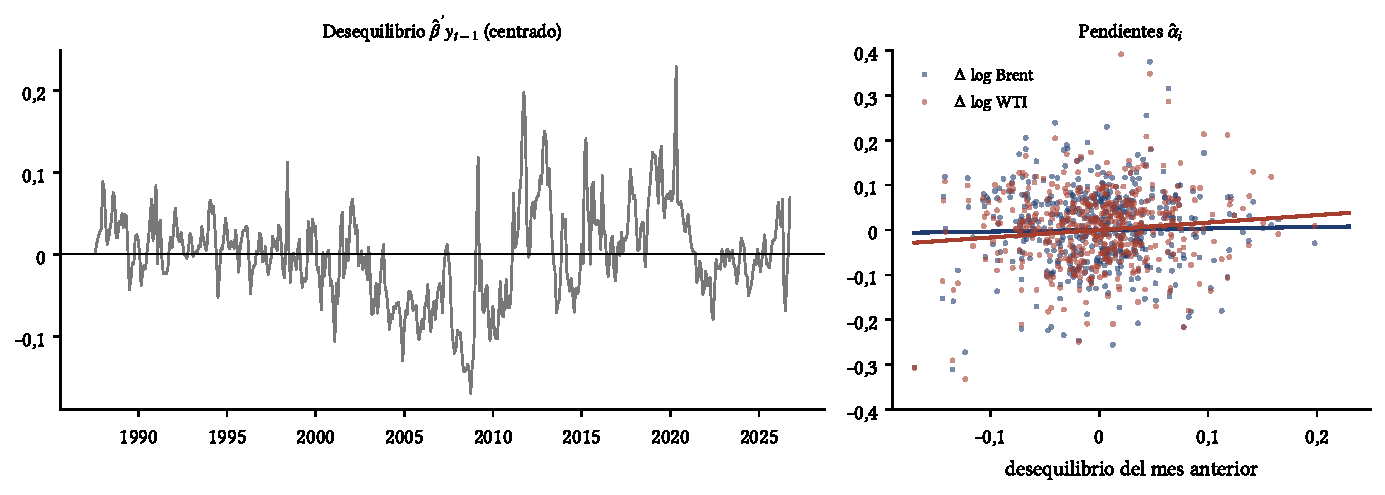
\includegraphics[width=\linewidth]{graficos/cap11_ej02_vecm.pdf}
\caption{Izquierda: desequilibrio estimado $\hat\beta'\mathbf y_{t-1}$, centrado. Derecha: cambio mensual de cada
precio frente al desequilibrio del mes anterior; las rectas tienen pendiente $\hat\alpha_i$, casi plana para el
Brent y positiva para el WTI.}
\label{fig:vecmpetro}
\end{figure}

\begin{conclusion}
Hay una relación de largo plazo entre el Brent y el WTI, y es el WTI el que se ajusta a ella. Pero la relación no es
de uno a uno en logaritmos durante toda la muestra.
\end{conclusion}
\end{ejresuelto}

\begin{ejresuelto}{El diferencial WTI-Brent y el cambio de régimen de 2011}\label{ej:regimen}
\enunciado Defina el diferencial $s_t=100(W_t-B_t)$, el precio del WTI respecto del Brent en porcentaje. Compare su
media y su estacionariedad, y las pruebas de Johansen, antes y después de enero de 2011.

\solucion
\paso{Paso 1. Dos regímenes.}
\begin{center}\small
\begin{tabular}{@{}lrrrrrr@{}}
\toprule
Período & $T$ & Media de $s_t$ & ADF de $s_t$ & Traza $r=0$ & $\hat\beta_{\text{WTI}}$ & $LR$: $\beta=(1,-1)'$ \\
\midrule
1987--2010 & 284 & 5,72 & $-2{,}66$ & 46,53 & $-1{,}048$ & 25,28 \\
2011--2026 & 190 & $-7{,}99$ & $-3{,}87$ & 22,88 & $-1{,}114$ & 6,12 \\
Completa   & 474 & 0,22 & $-1{,}74$ & 33,05 & $-1{,}112$ & 22,39 \\
\bottomrule
\end{tabular}
\end{center}
Hasta 2010 el WTI, un crudo más liviano y dulce, cotizaba en promedio 5,7\,\% por \emph{encima} del Brent. Desde
2011 cotiza 8,0\,\% por \emph{debajo}. En 2011--2013 la brecha promedió $-14{,}6$\,\% y llegó a $-27{,}7$\,\% en
septiembre de 2011 (Figura~\ref{fig:diferencial}). El aumento de la producción de crudo de esquisto en EE.\,UU.\
saturó la capacidad de almacenamiento y de oleoductos en Cushing (Oklahoma), donde se entrega el WTI, mientras que
el Brent seguía reflejando el mercado mundial. Cuando se construyeron nuevos oleoductos hacia la costa del
Golfo, la brecha se redujo, pero no volvió a su nivel anterior.

\paso{Paso 2. Lo que el cambio de media hace a las pruebas.} En la muestra completa el diferencial \emph{no} es
estacionario según la ADF ($-1{,}74$): una serie que fluctúa alrededor de dos medias distintas se parece a un
paseo aleatorio. Dentro de cada régimen la ADF es más negativa ($-2{,}66$, significativa al 10\,\% pero no al 5\,\%, y $-3{,}87$,
significativa al 1\,\%). Johansen encuentra cointegración en los tres casos, pero en la muestra completa lo hace
con $\hat\beta_{\text{WTI}}=-1{,}11$, lejos de uno: el $\beta$ se desvía para absorber el cambio de nivel.

\paso{Paso 3. Implicaciones.} Una relación de cointegración puede romperse por cambios estructurales en el
mercado. Con quiebres, las pruebas de raíz unitaria sobre el diferencial pierden potencia (como con el Brent en
el Capítulo~\ref{cap:raiz}) y el vector estimado se distorsiona. Para estos casos existen pruebas de cointegración
con quiebre endógeno, como la de Gregory y Hansen (1996).

\codigoweb{cap11_ej03}
\salidaR{cap11_ej03_R.txt}
\lectura{cap11_ej03}

\RvsPy Las submuestras se seleccionan comparando cadenas de fecha (\texttt{"2010-12"}), lo que funciona en los dos
lenguajes porque el formato \texttt{AAAA-MM} se ordena alfabéticamente igual que cronológicamente.

\begin{figure}[ht]
\centering
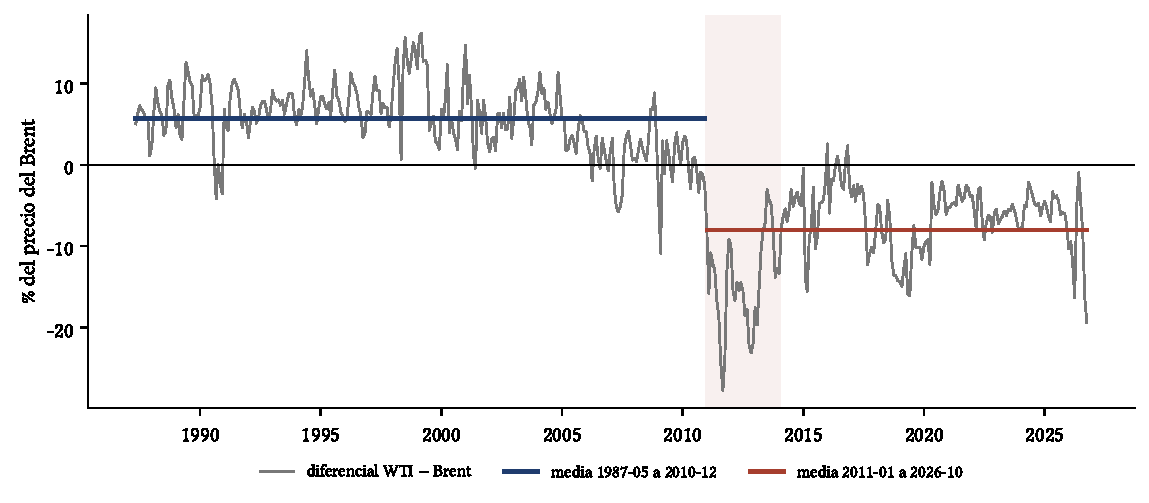
\includegraphics[width=0.92\linewidth]{graficos/cap11_ej03_diferencial.pdf}
\caption{Diferencial entre el WTI y el Brent en porcentaje, con la media de cada régimen. La franja sombreada marca
2011--2013, cuando la congestión en Cushing hundió el precio del WTI.}
\label{fig:diferencial}
\end{figure}

\begin{conclusion}
La ley de un solo precio entre el Brent y el WTI se cumple dentro de cada régimen, pero con un diferencial de
equilibrio que cambió de signo en 2011. Ignorar el quiebre lleva a un vector de cointegración distorsionado y a
pruebas engañosas sobre el diferencial.
\end{conclusion}
\end{ejresuelto}

\begin{ejresuelto}{El modelo de valor presente: precios, dividendos y utilidades}\label{ej:vp}
\enunciado Según el modelo de valor presente con tasa de descuento constante, el precio de una acción es
proporcional a sus dividendos esperados, y $\log(D_t/P_t)$ debería ser estacionario (Campbell y Shiller, 1987).
Con datos anuales reales del S\&P 500 (1871--2023), contraste la cointegración entre $\log P$ y $\log D$, y entre
$\log P$ y $\log E$ (utilidades).

\solucion
\paso{Paso 1. Raíces unitarias.}
\begin{center}\small
\begin{tabular}{@{}lrrrrr@{}}
\toprule
 & $\log P$ & $\log D$ & $\log E$ & $\log(D/P)$ & $\log(E/P)$ \\
\midrule
ADF ($t$) & $-0{,}31$ & $-0{,}43$ & 0,70 & $-1{,}41$ & $-4{,}66$ \\
\bottomrule
\end{tabular}
\end{center}
Los tres niveles son I(1). La razón utilidad/precio es claramente estacionaria, pero la razón dividendo/precio
no lo es.

\paso{Paso 2. Johansen.}
\begin{center}\small
\begin{tabular}{@{}lrrrrr@{}}
\toprule
Par & Traza $r=0$ & $\hat\beta$ & $t(\hat\alpha_P)$ & $t(\hat\alpha_X)$ & $LR$: $\beta=(1,-1)'$ \\
\midrule
$P$ y $D$ ($k=1$) & 21,21 & $(1;\ -1{,}720)$ & $-0{,}96$ & 4,39 & 17,51 \\
$P$ y $E$ ($k=0$) & 33,32 & $(1;\ -1{,}285)$ & 0,19 & 5,66 & 10,91 \\
\bottomrule
\end{tabular}
\end{center}
En ambos pares la traza rechaza $r=0$ (valor crítico 15,49), pero $\beta=(1,-1)'$ se rechaza también. Y quien
corrige el desequilibrio no es el precio, sino los dividendos y las utilidades ($\hat\alpha_X$ significativos,
$\hat\alpha_P$ no): cuando los precios están altos respecto de los dividendos, son los dividendos los que tienden a
subir después, no los precios los que bajan.

\paso{Paso 3. ¿Por qué no es estacionario $\log(D/P)$?} La razón dividendo/precio pasó de 5,86\,\% en 1871 a
1,70\,\% en 2023 (Figura~\ref{fig:vp}). Parte de la caída se debe a un cambio en la política de pagos: las empresas
repartían en promedio el 70,2\,\% de sus utilidades como dividendos entre 1871 y 1950, pero solo el 48,9\,\% entre
1990 y 2023, porque hoy devuelven efectivo a sus accionistas sobre todo recomprando acciones. Las utilidades no
tienen ese problema, y $\log(E/P)$ sí resulta estacionario.

\codigoweb{cap11_ej04}
\salidaR{cap11_ej04_R.txt}
\lectura{cap11_ej04}

\RvsPy Con $k=0$ no hay rezagos de las diferencias y la matriz de regresores auxiliares contiene solo la
constante. En R, \texttt{cbind(1, NULL)} produce una matriz $1\times1$ y no un vector columna de unos, lo que
rompía los productos matriciales; la función usa \texttt{matrix(1, n, 1)}. En Python, \texttt{np.column\_stack}
con una sola columna no tiene ese problema.

\begin{figure}[ht]
\centering
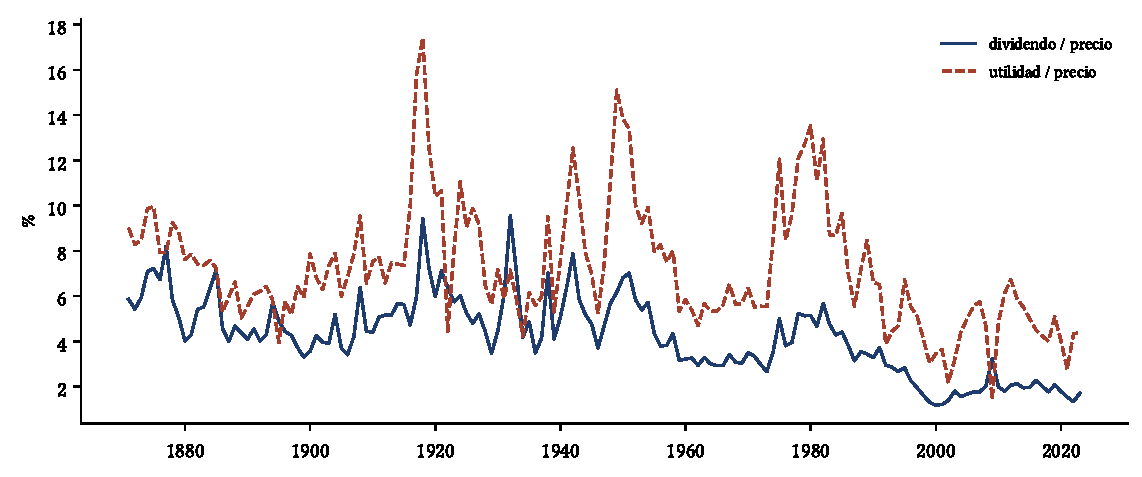
\includegraphics[width=0.92\linewidth]{graficos/cap11_ej04_valor_presente.pdf}
\caption{Razones dividendo/precio y utilidad/precio del S\&P 500 (enero de cada año, 1871--2023). La primera tiene
una tendencia descendente; la segunda fluctúa alrededor de un nivel estable.}
\label{fig:vp}
\end{figure}

\begin{conclusion}
Precios, dividendos y utilidades comparten una tendencia de largo plazo, pero la relación no es la proporcional
que supone el modelo de valor presente más simple, sobre todo para los dividendos. Y el ajuste lo hacen los
fundamentos, no los precios: los precios altos anuncian dividendos más altos, no caídas de precio, un resultado
que debe leerse con cautela porque los cambios en la política de pagos rompen la estacionariedad de $D/P$.
\end{conclusion}
\end{ejresuelto}

\begin{ejresuelto}{¿Ayuda la corrección de errores a pronosticar?}\label{ej:vecmpron}
\enunciado Pronostique el cambio mensual de $\log$ Brent y $\log$ WTI desde enero de 2005, con ventana creciente,
usando un paseo aleatorio, un VAR(2) en diferencias y el VECM con $k=2$ y $r=1$ (reestimando $\beta$ en cada mes).
Compare la raíz del error cuadrático medio (RECM) y aplique la prueba de Clark y West del VAR en diferencias
(anidado, con $\alpha=0$) frente al VECM.

\solucion
\paso{Paso 1. Errores.} Con 262 pronósticos:
\begin{center}\small
\begin{tabular}{@{}lrrr@{}}
\toprule
RECM (\%) & Paseo aleatorio & VAR en diferencias & VECM \\
\midrule
Brent & 10,776 & 10,415 & 10,546 \\
WTI   & 10,728 & 10,504 & 10,537 \\
\bottomrule
\end{tabular}
\end{center}
Los dos modelos dinámicos superan al paseo aleatorio (en parte por el efecto Working que introduce promediar los
precios), pero el VECM no supera al VAR en diferencias.

\paso{Paso 2. Clark y West.} Para el Brent, $t=-1{,}73$ ($p=0{,}96$); para el WTI, $t=0{,}11$ ($p=0{,}46$). La
corrección de errores no mejora los pronósticos a un mes, y su $R^2$ fuera de muestra respecto del VAR en
diferencias es negativo ($-2{,}54$\,\% y $-0{,}63$\,\%).

\paso{Paso 3. ¿Por qué?} La Figura~\ref{fig:vecmpron} muestra que el VECM acumula casi toda su desventaja en dos
episodios: el derrumbe de fines de 2008 y la anomalía de abril de 2020. En ambos, el desequilibrio fue enorme y el
modelo predijo una corrección fuerte que no llegó al mes siguiente. Además, $\hat\beta$ cambia con el quiebre de
2011. Christoffersen y Diebold (1998) muestran que la cointegración ayuda sobre todo a pronosticar a horizontes
largos, y no tanto a un mes, cuando dominan los choques de corto plazo.

\codigoweb{cap11_ej05}
\salidaR{cap11_ej05_R.txt}
\lectura{cap11_ej05}

\RvsPy El pronóstico del VECM es el producto del vector $(\hat\beta'\mathbf y_{t-1},\,1,\,\Delta\mathbf y_{t-1}',\,
\Delta\mathbf y_{t-2}')$ por la matriz de coeficientes estimada; el del VAR en diferencias usa el mismo vector sin el
primer elemento. Como Python indexa desde cero, el cambio del mes $t$ es \texttt{dYall[t-1]}; en R es
\texttt{diff(L)[t - 1, ]} con $t$ contado desde uno. Ambos dan idénticos resultados.

\begin{figure}[ht]
\centering
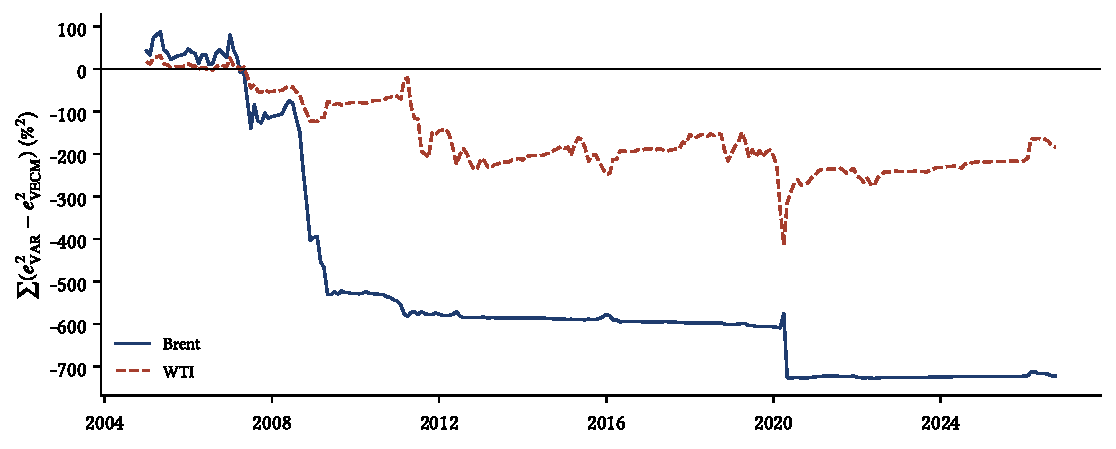
\includegraphics[width=0.88\linewidth]{graficos/cap11_ej05_pronostico.pdf}
\caption{Diferencia acumulada entre los errores cuadráticos del VAR en diferencias y los del VECM. Una curva que
baja indica que el VECM pronostica peor; las caídas se concentran en 2008 y 2020.}
\label{fig:vecmpron}
\end{figure}

\begin{conclusion}
Que dos precios estén cointegrados no garantiza que el modelo de corrección de errores pronostique mejor a corto
plazo. Con quiebres estructurales y choques extremos, el término de corrección puede incluso empeorar el
pronóstico.
\end{conclusion}
\end{ejresuelto}

% ---------------------------------------------------------------------
\section{Ejercicios propuestos}
% ---------------------------------------------------------------------

\begin{enumerate}[label=\textbf{\thechapter.\arabic*},leftmargin=*,itemsep=6pt]
  \item Escriba el VECM de un VAR(3) y exprese $\Gamma_1$ y $\Gamma_2$ en función de $A_1$, $A_2$ y $A_3$.
  \textit{Respuesta: $\Gamma_1=-(A_2+A_3)$, $\Gamma_2=-A_3$.}

  \item En un VECM bivariado sin rezagos con $\beta=(1,-1)'$ y $\alpha=(-0{,}1;\ 0{,}1)$, calcule el coeficiente
  autorregresivo del desequilibrio, su vida media y el nivel final tras un choque $\mathbf y_0=(1,0)'$.
  \textit{Respuesta: $0{,}8$; $3{,}1$ períodos; $0{,}5$.}

  \item Demuestre que si $\Pi=\alpha\beta'$ con $\alpha$ y $\beta$ de dimensión $K\times r$, entonces
  $\operatorname{rango}(\Pi)\le r$.

  \item Con autovalores $\hat\lambda=(0{,}10;\ 0{,}02)$ y $n=300$, calcule los estadísticos de la traza y del máximo
  autovalor y decida el rango con los valores críticos del texto. \textit{Respuesta: traza $37{,}67$ y $6{,}06$;
  máximo $31{,}61$ y $6{,}06$; rango 2, es decir, ambas series serían estacionarias.}

  \item \emph{(Simulación.)} Simule 2\,000 pares de paseos aleatorios independientes con $T=200$, aplique la prueba
  de Engle y Granger y compare la frecuencia de rechazos con los valores críticos de Dickey-Fuller ($-2{,}86$) y de
  MacKinnon ($-3{,}37$ para $T=200$). ¿Cuál tiene el tamaño correcto?

  \item \emph{(Con datos del BCRP.)} Contraste la cointegración entre el tipo de cambio sol/dólar y el índice de
  precios relativos Perú/EE.\,UU. (paridad del poder de compra). ¿Qué variable corrige?

  \item \emph{(Con datos.)} Repita el Ejercicio~\ref{ej:johansen} solo para 2011--2026 e interprete $\hat\alpha$.
  ¿Sigue siendo el Brent débilmente exógeno?

  \item \emph{(Con datos de Yahoo Finance.)} Descargue los precios diarios de dos acciones del mismo sector (por
  ejemplo, dos bancos). Contraste la cointegración en 2015--2020 y use el residuo estandarizado como señal de una
  estrategia de \emph{pairs trading} en 2021--2025. ¿Se mantiene la relación fuera de la muestra?
\end{enumerate}

% ---------------------------------------------------------------------
\section{Resumen de fórmulas}
% ---------------------------------------------------------------------

\begin{table}[H]
\centering\small
\begin{tabular}{@{}ll@{}}
\toprule
Concepto & Fórmula \\
\midrule
VECM & $\Delta\mathbf y_t=\mathbf c+\alpha\beta'\mathbf y_{t-1}+\sum_{i=1}^{p-1}\Gamma_i\Delta\mathbf y_{t-i}+\mathbf u_t$ \\
Matrices & $\Pi=-(I-\sum_jA_j)=\alpha\beta'$;\quad $\Gamma_i=-\sum_{j>i}A_j$ \\
Desequilibrio & $z_t=\beta'\mathbf y_t$;\quad persistencia $1+\beta'\alpha$ (sin rezagos) \\
Engle-Granger & ADF sin constante sobre $\hat u_t$;\quad VC 5\,\%: $-3{,}336-6{,}11/T-6{,}82/T^2$ \\
Johansen & autovalores de $S_{11}^{-1}S_{10}S_{00}^{-1}S_{01}$ \\
Traza & $-n\sum_{i=r+1}^{K}\ln(1-\hat\lambda_i)$ \\
Máximo autovalor & $-n\ln(1-\hat\lambda_{r+1})$ \\
Restricción $\beta=H\varphi$ & $n[\ln(1-\tilde\lambda_1)-\ln(1-\hat\lambda_1)]\sim\chi^2_{K-s}$ \\
\bottomrule
\end{tabular}
\caption{Fórmulas principales del Capítulo 11.}
\end{table}

\section*{Referencias}
\begin{itemize}[leftmargin=*]
  \item Campbell, J. Y. y Shiller, R. J. (1987). Cointegration and tests of present value models. \emph{Journal of
        Political Economy}, 95(5), 1062--1088.
  \item Christoffersen, P. F. y Diebold, F. X. (1998). Cointegration and long-horizon forecasting. \emph{Journal of
        Business \& Economic Statistics}, 16(4), 450--458.
  \item Engle, R. F. y Granger, C. W. J. (1987). Co-integration and error correction: Representation, estimation,
        and testing. \emph{Econometrica}, 55(2), 251--276.
  \item Gregory, A. W. y Hansen, B. E. (1996). Residual-based tests for cointegration in models with regime
        shifts. \emph{Journal of Econometrics}, 70(1), 99--126.
  \item Johansen, S. (1988). Statistical analysis of cointegration vectors. \emph{Journal of Economic Dynamics and
        Control}, 12(2--3), 231--254.
  \item Johansen, S. (1991). Estimation and hypothesis testing of cointegration vectors in Gaussian vector
        autoregressive models. \emph{Econometrica}, 59(6), 1551--1580.
  \item MacKinnon, J. G. (2010). Critical values for cointegration tests. Queen's Economics Department Working
        Paper 1227.
  \item MacKinnon, J. G., Haug, A. A. y Michelis, L. (1999). Numerical distribution functions of likelihood ratio
        tests for cointegration. \emph{Journal of Applied Econometrics}, 14(5), 563--577.
\end{itemize}
